\section{Architecture neuronal}
Une fois la structure du modèle définie (Actor,critic), il nous faut définir les structures des réseaux neuronaux.
En effet, pour un problème donné, certaines structures sont plus adaptées que d’autres.
Nous avons utilisé 3 structures différentes :

\begin{itemize}
    \item ANN simple ( Artificial Neural Network)
    \item RNN ( Recurrent Neural Network)
    \item CNN (Convolutional Neural Network)
\end{itemize}

\subsection{ANN}

\begin{figure}[H]
    \centering
    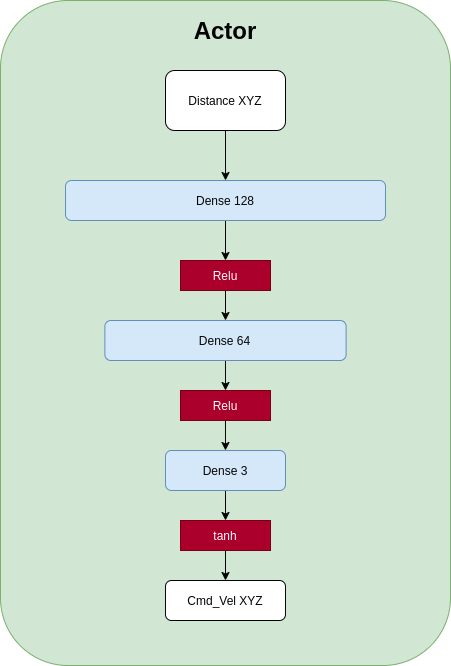
\includegraphics[width=0.5\textwidth]{./image_RL/image40.png}
    \caption{Actor}
\end{figure}

\begin{figure}[H]
    \centering
    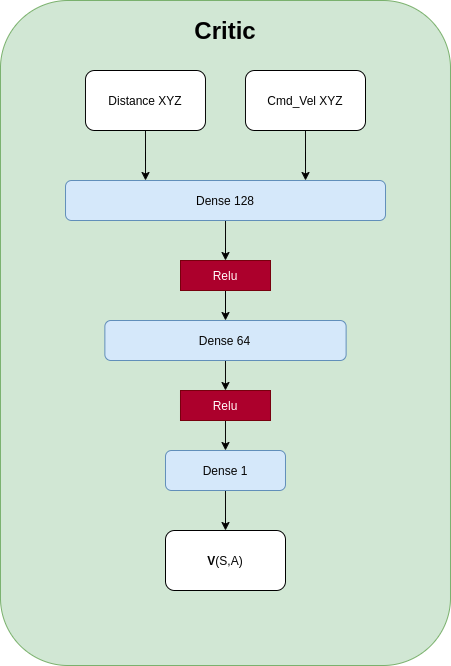
\includegraphics[width=0.5\textwidth]{./image_RL/image15.png}
    \caption{Critic}
\end{figure}

Comme on peut le voir, le réseau se compose principalement de deux entités.
Les denses correspondent aux layers du réseau de neurones. Chaque couche contient un nombre défini de neurones [6].
Les fonctions d’activations en rouge, représentent la fonction par laquelle passe la sortie du neurone.
Ici on retrouve principalement 2 fonctions d’activations:

Relu :
\begin{figure}[H]
    \centering
    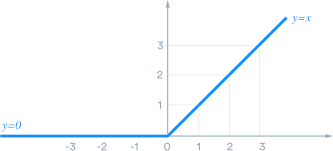
\includegraphics[width=0.5\textwidth]{./image_RL/image34.png}
    \caption{Fonction Relu}
\end{figure}

La fonction d'activation la plus utilisée de nos jours est la ReLU - Rectified Linear Unit - qui est une fonction linéaire par morceaux. Son avantage réside sur le fait qu'elle remplace toute valeur d'entrée négative par 0 et toute valeur positive par elle-même. Pour son gradient, il devient nul pour les valeurs négatives et vaut 1 pour les valeurs positives. Cette propriété est très intéressante dans la phase d'apprentissage car elle permet “d’éteindre” certains neurones et donc de permettre au réseau de se “spécialiser” dans certains domaines. De plus, cela permet de réduire significativement l'entraînement.
Tanh:
\begin{figure}[H]
    \centering
    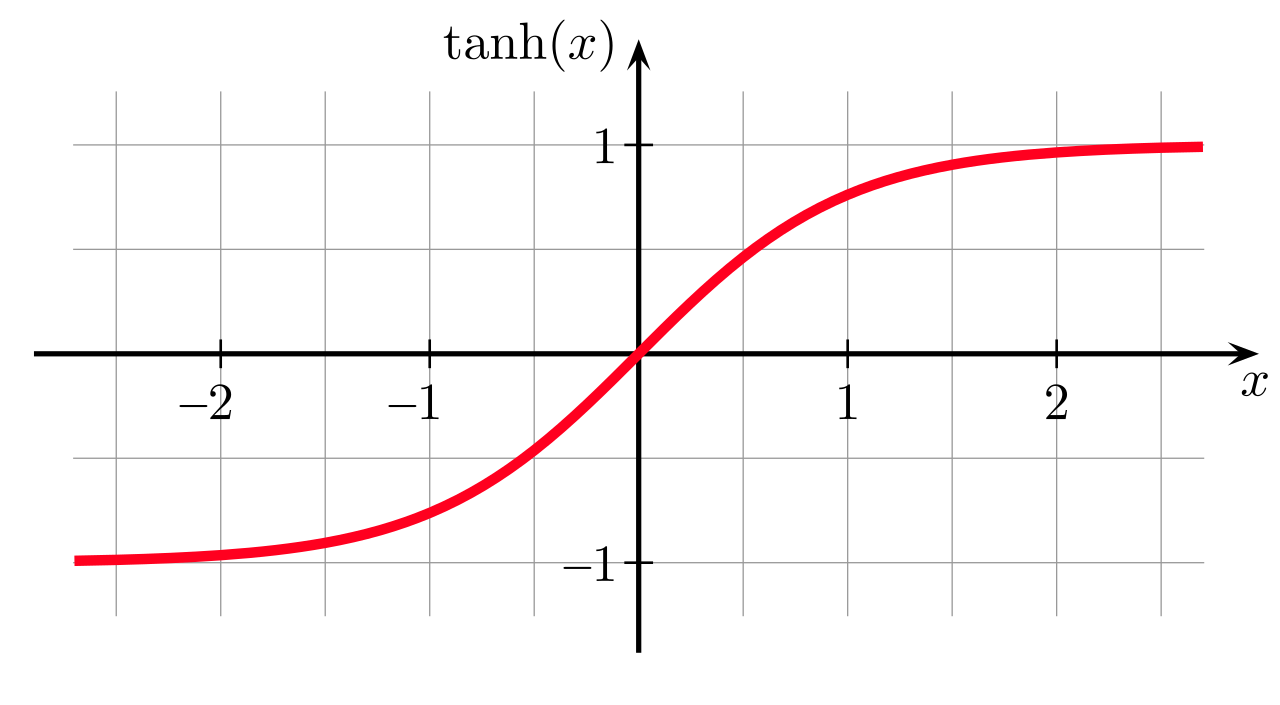
\includegraphics[width=0.5\textwidth]{./image_RL/image8.png}
    \caption{Fonction Tanh}
\end{figure}

On utilise donc la fonction d’activation tangente hyperbolique en sortie du réseau ce qui permet d’obtenir une sortir entre -1 et 1 que l’on rescale en multipliant par les bornes physiques du système (commande maximales)

\subsection{RNN}

Les réseaux de neurones récurrents ont une structure particulière. En effet, elle permet d’utiliser comme entrée une série de données. Dans le premier réseau de neurones, nous donnions en entrée les distances sur X, Y, Z séparant le drone de sa cible.
Or une donnée pouvant apporter de l’information est bien sûr la vitesse.
Il y a donc deux possibilités. La première est d'utiliser un réseau de neurones simple et de calculer la vitesse du drone dans le repère de la cible ce qui peut être sujet à une accumulation d’incertitudes dû aux différents capteurs utilisés.
Ou bien déduire d’une série de données la vitesse du drone.
Nous avons choisi la deuxième solution. 

En effet, il existe des structures de réseaux qui permettent de déduire d’une série temporelle de données des informations quant à l’évolution temporelle du système.

C’est le cas des LSTM pour Long Short Term Memory. Ces réseaux complex se démarque de part leur architecture spécifique :

\begin{figure}[H]
    \centering
    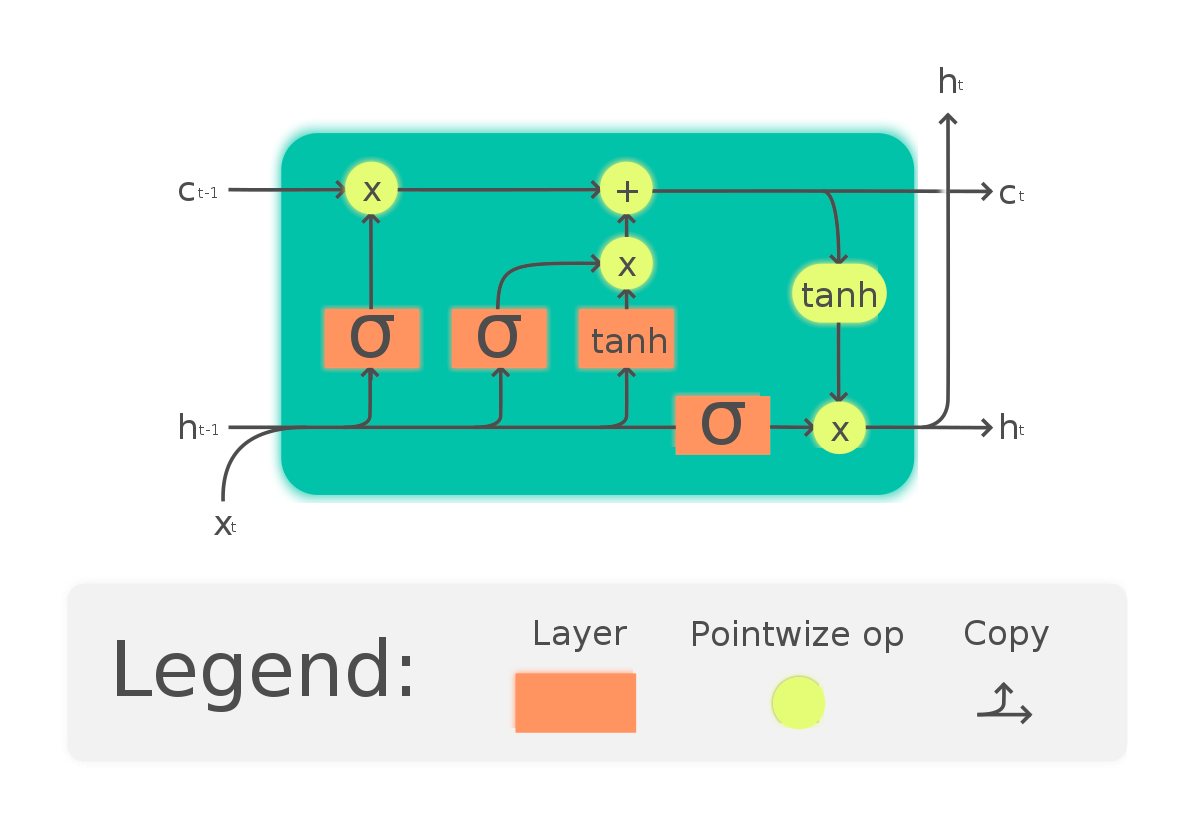
\includegraphics[width=0.5\textwidth]{./image_RL/image26.png}
    \caption{Structure LSTM}
\end{figure}

Le fonction de ces réseau est expliquée de façon exhaustive dans l’article [7].
Synthétiquement, on observe une ligne principale C qui compose la ligne temporelle d’information. En effet, à chaque passage dans le réseau, il faut renseigner C qui comporte l’information qu'a stocké le réseau jusqu’ici. Le réseau met à jour l’information à stocker en fonction de ce qu'il considère important ou non à retenir. Pour faire son choix, il utilise la sortie précédente H(t-1) et l’état courant Xt.
Il faut donc définir la taille de la série sur laquelle nous allons entraîner notre réseau. Nous avons utilisé des séries de 4 états.
En sortie de la couche LSTM, on place un simple réseau de neurones pour interpréter cette sortie.
On a donc pour l’actor la structure suivante :

\begin{figure}[H]
    \centering
    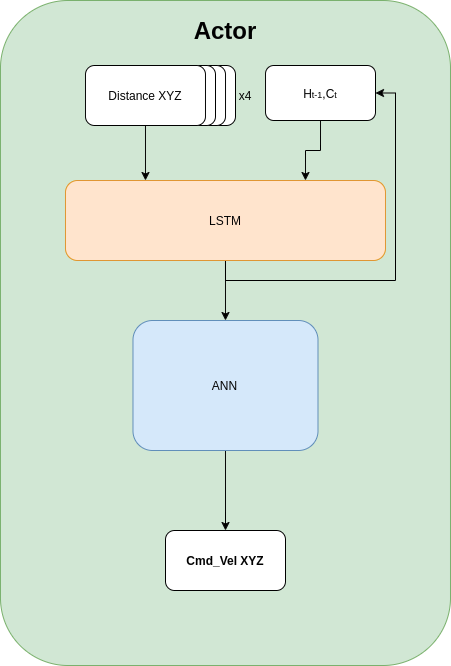
\includegraphics[width=0.5\textwidth]{./image_RL/image17.png}
    \caption{Structure Actor with LSTM}
\end{figure}

\subsection{CNN}

CNN pour Convolutional Neural Network. Ces réseaux sont aujourd’hui bien connus dans le milieu du deep learning si bien qu'ils sont devenus indispensables pour les problèmes de classifications d’images.
Ces réseaux ont des performances remarquables pour extraire l’information d’une image.
Dans notre cas de figure, le drone est équipé d’une caméra placée dessous qui permet d’avoir un retour image sur la scène.
Dans la phase d'atterrissage on peut considérer que si la plateforme sur laquelle on doit se poser reste dans le champ de vision de la caméra à chaque instant, l’image est une donnée nécessaire et suffisante pour caractériser l’état de l’agent.

On peut alors tenter d’asservir le robot seulement grâce au retour image.
Le réseau prend en entrée l’image et ressort une commande Cmdvel.
Le fonction des réseaux de neurones à convolution est expliqué dans [8].
Un réseau de neurones à convolution ont la structure suivante :
\begin{figure}[H]
    \centering
    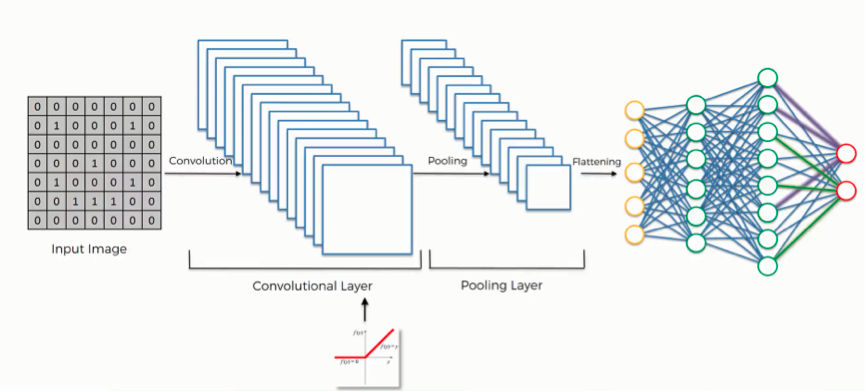
\includegraphics[width=0.5\textwidth]{./image_RL/image46.png}
    \caption{Convolutional Neural Network  }
\end{figure}

On remarque qu’en amont du réseau de neurone, on ajoute une couche de convolution et de pooling qui permettent d’extraire les “features” (informations) de l’image. 
(Sur l’image une seule couche est représentée mais usuellement plusieurs couches sont utilisées.)
La couche de convolution permet elle véritablement d’extraire l’information, alors que la couche de pooling consiste à un subsample qui permet de réduire la dimension du layer d’entrée dans le réseau de neurones.
L’étape de flattening consiste à récupérer tous les coefficients qui ressortent de la couche de convolution et pooling et à les stocker dans un seul et même vecteur.
En effet, plus on a une dimension élevée pour le layer d'entrée, plus il faut un réseau profond pour interpréter l’image et plus le réseau est long à entraîner.

Dans notre cas on ainsi la structure suivante pour l’actor :

\begin{figure}[H]
    \centering
    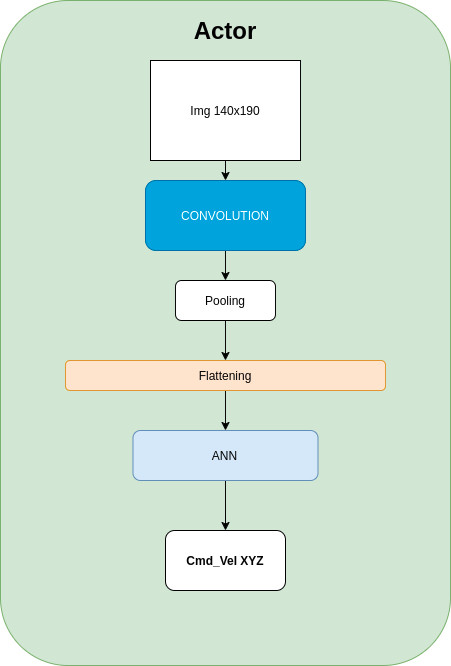
\includegraphics[width=0.5\textwidth]{./image_RL/image21.png}
    \caption{ Actor with CNN }
\end{figure}